%

% Cal Poly Thesis
% 
% based on UC Thesis format
%
% modified by Mark Barry 2/07.
%




\documentclass[12pt]{ucthesis}



\newif\ifpdf
\ifx\pdfoutput\undefined
    \pdffalse % we are not running PDFLaTeX
\else
\pdfoutput=1 % we are running PDFLaTeX
\pdftrue \fi

\usepackage{url}
\ifpdf

    \usepackage[pdftex]{graphicx}
    % Update title and author below...
    \usepackage[pdftex,plainpages=false,breaklinks=true,colorlinks=true,urlcolor=blue,citecolor=blue,%
                                       linkcolor=blue,bookmarks=true,bookmarksopen=true,%
                                       bookmarksopenlevel=3,pdfstartview=FitV,
                                       pdfauthor={!!Author goes here!!},
                                       pdftitle={!!Title goes here!!},
                                       pdfkeywords={thesis, masters, cal poly}
                                       ]{hyperref}
    %Options with pdfstartview are FitV, FitB and FitH
    \pdfcompresslevel=1

\else
    \usepackage{graphicx}
\fi

\graphicspath{ {Images/} }

\usepackage{longtable}
\usepackage{amssymb}
\usepackage{amsmath}
\usepackage[letterpaper]{geometry}
\usepackage[overload]{textcase}

%\usepackage[disable]{todonotes} % notes not showed
\usepackage[draft]{todonotes}   % notes showed

\bibliographystyle{abbrv}

\setlength{\parindent}{0.25in} \setlength{\parskip}{6pt}

\geometry{verbose,nohead,tmargin=1.25in,bmargin=1in,lmargin=1.5in,rmargin=1.3in}

\setcounter{tocdepth}{2}


% Different font in captions (single-spaced, bold) ------------
\newcommand{\captionfonts}{\small\bf\ssp}

\makeatletter  % Allow the use of @ in command names
\long\def\@makecaption#1#2{%
  \vskip\abovecaptionskip
  \sbox\@tempboxa{{\captionfonts #1: #2}}%
  \ifdim \wd\@tempboxa >\hsize
    {\captionfonts #1: #2\par}
  \else
    \hbox to\hsize{\hfil\box\@tempboxa\hfil}%
  \fi
  \vskip\belowcaptionskip}
\makeatother   % Cancel the effect of \makeatletter
% ---------------------------------------




\begin{document}

% Declarations for Front Matter

% Update fields below!
\title{Detecting Zebra Crosswalks Using Neural Networks}
\author{Jason Banich}
\degreemonth{March} \degreeyear{2016} \degree{Master of Science}
\defensemonth{March} \defenseyear{2016}
\numberofmembers{3} \chair{Dr. John Seng} \othermemberA{Dr. Franz Kurfess} \othermemberB{Person3, Ph.D.} \campus{San Luis Obispo}
\copyrightyears{seven}


\todo[inline]{COMMMENTS ARE ENABLED THIS IS NOT THE FINAL VERSION}
\todo[inline]{BE SURE THAT STRIPLETS HAS BEEN FIND AND REPLACED TO STRIPELETS FOR FINAL - CHECK CASE}

\maketitle

\begin{frontmatter}

% Custom made for Cal Poly (by Mark Barry, modified by Andrew Tsui).
\copyrightpage

% Custom made for Cal Poly (by Andrew Tsui).
\committeemembershippage

\begin{abstract}
It can be difficult to guide yourself across a crosswalk successfully when your visual capabilities are limited. This can be an everyday issue for someone with impaired vision. This paper aims to help alleviate that issue by focusing on zebra stripe crosswalks and coming up with an algorithm that can quickly and accurately identify and help guide a user across the crosswalk using a handheld device such as a phone. \todo[inline]{NOT ACTUALLY A PHONE APP}The image is identified as being part of a crosswalk or not, and then the user could be given feedback directing them back towards the crosswalk if they are off-course.

\todo[inline]{Add more/redo}

\end{abstract}

\begin{acknowledgements}
I would like to acknowledge my parents for supporting me through college.
\todo[inline]{Actually write this}
\end{acknowledgements}


\tableofcontents


\listoftables

\listoffigures

\end{frontmatter}

\pagestyle{plain}




\renewcommand{\baselinestretch}{1.66}


% ------------- Main chapters here --------------------





\chapter{Introduction}
\label{intro}

Crossing the street can be very dangerous for visually impaired individuals. Orienting oneself is difficult without vision. Visually impaired people must use other cues such as listening for cars stopped at red lights and trying to walk in front of them. Vision processing could be applied to recognize the crosswalk to assist the user with limited vision. In order to increase the safety of blindly crossing the street, a phone app could allow the user to hold up their phone and get feedback about the location of the crosswalk. As they cross the street, they would receive feedback as to whether they were going off course. Developing a fast and reliable metric for detecting the crosswalk is the first step towards developing a vision processing phone app to aid the visually impaired.

There have been some investigations of the zebra crosswalk detection already, but none so far have used neural networks \todo[inline]{citations of some papers}. Neural networks are formed by a number of interconnected nodes that require training. Once trained, they can be configured to a specific application to predict outcomes based on the inputs. Neural networks are being used for an increasing number of applications where patterns are very hard to decipher manually. Although the training process can be time consuming, neural networks run very quickly once trained, which is a large benefit to any application where speed is a factor. 

Figure-ground segmentation has been used to separate the objects from the background scene. This technique can be applied to zebra crosswalks to allow the detection of potential stripelets in the image using geometric parameters \cite{coughlan2006}. Adding neural networks to this discovery method allows us to use parameters that could be very difficult to manually train to help to decide whether potential stripelets are truly a part of a crosswalk or not. This paper aims to use neural networks to improve the reliability of zebra crosswalk detection methods, by offering a different approach to the problem.

\todo[inline]{-brief intro of NN-, explain basis of paper this is based on, explain training process, explain stripelets a bit, training parameters, one line about results, figure ground segmentation}

\todo[inline]{Introductory Paragraph - 
State the general field of interest in one or two paragraphs, and end with a sentence that states what study will accomplish. Do not keep the reader waiting to find out the precise subject of the dissertation.

Explain your goals.

overview of what will present}

\chapter{Background}
\section{Types of crosswalks}

There are many types of crosswalks (See figure \ref{fig:TypesOfXwalksFig} and \ref{fig:TypesOfXwalksRealFig} for some examples), with the main two being zebra stripe crosswalks and standard two line crosswalks. Two line crosswalks are more commonly used due to their simplicity, but zebra crosswalks are often used in more critical intersections due to their benefits in visibility \cite{crosswalkTypeEvaluation}. Using vision processing to recognize the boundaries of two line crosswalks has essentially been done many times over, because there is no real difference between processing a two line crosswalk and processing the driving lane of a car.

\begin{figure}[h]
\begin{center}
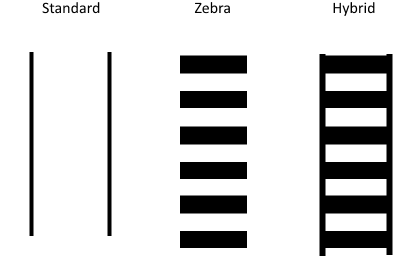
\includegraphics[width=10cm]{TypesOfXwalks.png}
\captionfonts
\caption[This is a figure]{A few types of crosswalks}
\label{fig:TypesOfXwalksFig}
\end{center}
\end{figure}

\begin{figure}[h]
\begin{center}
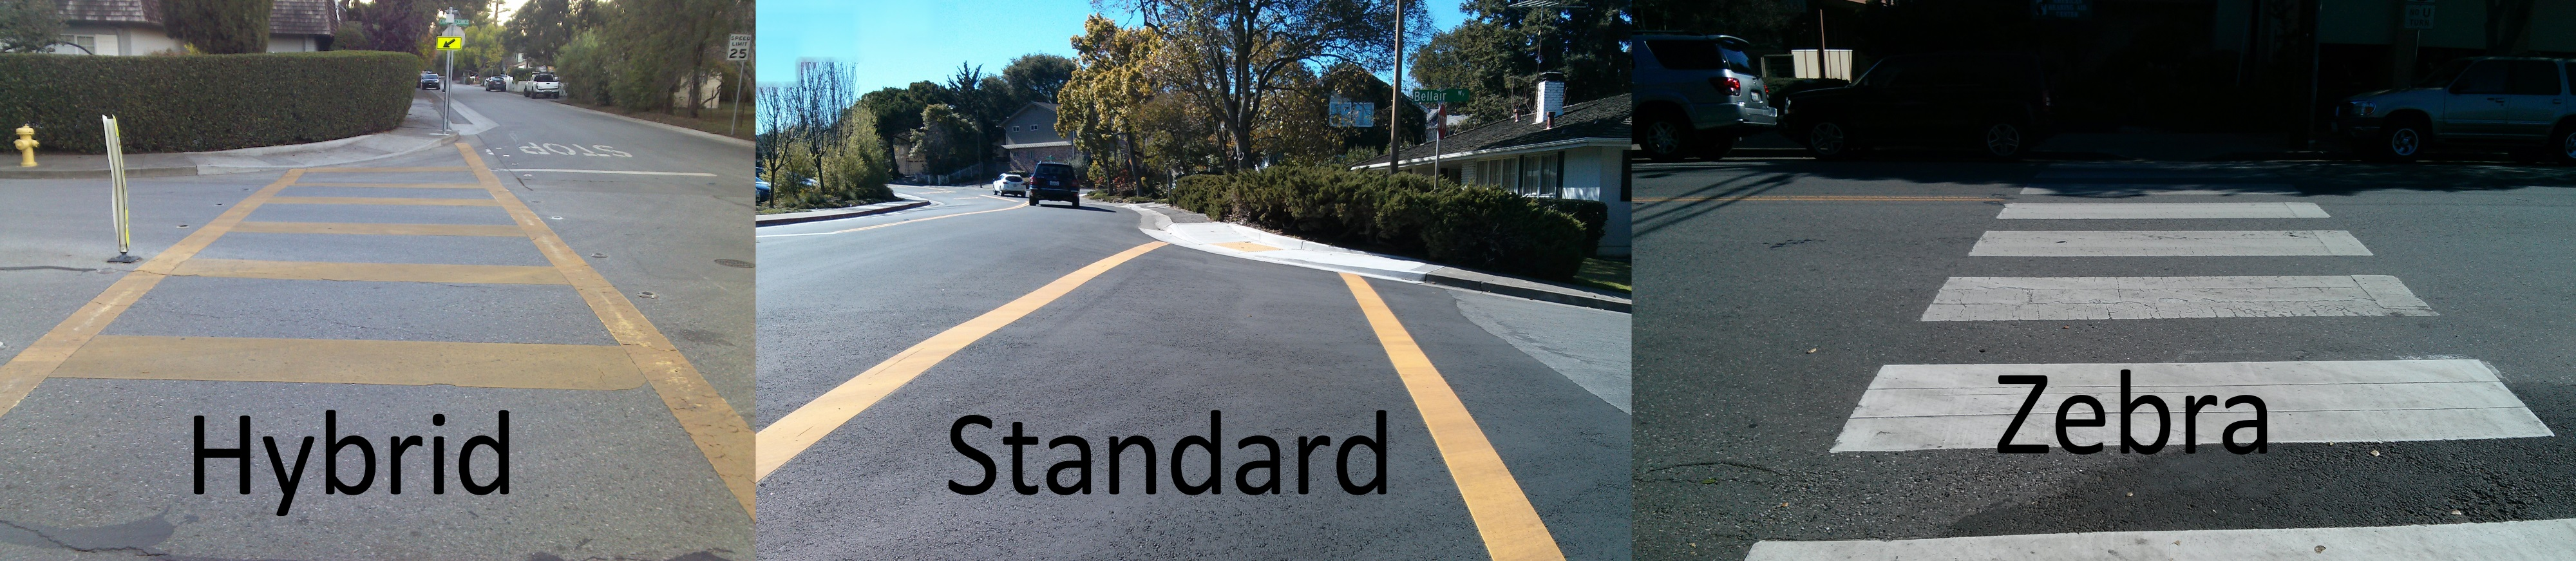
\includegraphics[width=13cm]{All3Types.jpg}
\captionfonts
\caption[This is a figure]{Real world samples of the types of crosswalks}
\label{fig:TypesOfXwalksRealFig}
\end{center}
\end{figure}

\section{Neural Networks}
Neural network are a type of machine learning that has been used recently for many vision applications such as image classification (See figure \ref{fig:DogWithHat}) and pattern recognition \cite{christianszegedy2014}. Neural networks function using an interconnected network of neurons that work together to process the training data in order to discover a pattern or classification. Neural networks are well suited for many data sets that include lots of information that could be very difficult to manually train a computer to categorize. They can even be used to help determine what signals from the brain to use to trigger prosthetic limbs to move by measuring results of brain probes in rats \cite{ratNeural}.

Neural networks are given a large amount of training data with known outputs. The network then runs over the entire dataset repeatedly, adjusting weighting parameters of each of the inputs each time to reduce the amount of error in the predictions, as well as backpropogation of the data in order to assist in training. Once the neural network is trained, the application can feed in newly discovered values and receive a prediction of the output.  

\todo[inline]{this paragraph needs a strong rework}

\begin{figure}[h]
\begin{center}
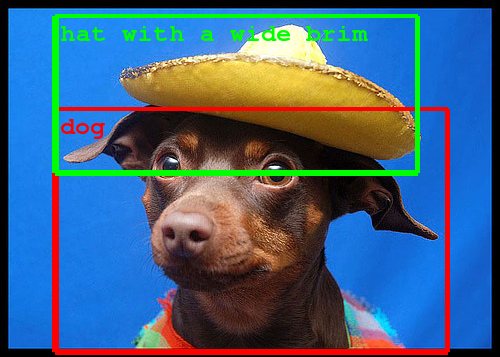
\includegraphics[width=10cm]{DogWithHat.PNG}
\captionfonts
\caption[This is a figure]{Neural network classification result\cite{christianszegedy2014}}
\label{fig:DogWithHat}
\end{center}
\end{figure}

\section{OpenCV}
\todo[inline]{WRITE THiS? where does it go?}

\chapter{Related Works}
\label{Related Works}

\section{Zebra Crosswalk Detection Using Cell Phone}

\begin{figure}[htp]
  \centering
  \begin{center}
    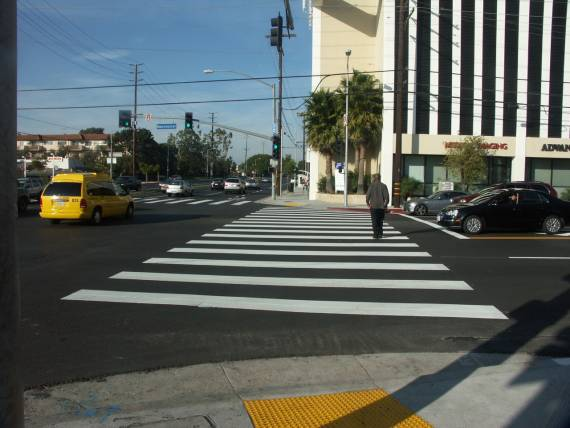
\includegraphics[width=0.45\textwidth]{Zebra.jpg}
    \caption{Zebra Crosswalk}
    \label{fig:Zebra}
  \end{center}
\end{figure}

\paragraph{}
One method for detecting zebra crosswalks was tested in ``Detecting and locating crosswalks using a camera phone\cite{ZebraPhone}.'' The authors proposed a method based on a few steps:
\begin{enumerate}
  \item Extract straight line segments from the image
  \item Apply segmentation algorithm to group the detected segments
  \item Score the detected segments using factor graphs
  \item Use a predetermined threshold to determine if there are enough highly scored horizontal line segments in the image to classify it as a crosswalk or not
\end{enumerate}

They were able to attain 'true positive' rates of 72\% and 'false positive' rates  of 0.5\% of determining whether the line segments were part of a crosswalk using this method. 


\section{Simple Lane Following Algorithm}
\paragraph{}
As autonomous cars start to become a reality, there are needs for algorithms
that can assist them in navigating and staying inside the lines. These
algorithms work by detecting the lines that are drawn on the pavement, and
instructing the car to stay in the center of these two lines. This is similar to
the crosswalk problem, in that you want the user to stay in between the two
lines, but different because you don't necessarily want the user to stay in the
precise center at all times, the main goal is to keep them inside the crosswalk.
One algorithm for lane following is as follows:
\begin{enumerate}
  \item Convert the image to grayscale
  \item Crop to the center portion of the image
  \item Identify the edges using an edge detection algorithm, and then draw the
  edges onto a new image
  \item Apply Hough line detection to find shapes in the edges
  \item Delete extraneous lines that were detected
  \item Reapply the lines that have been found to the main image and draw them
  on
\end{enumerate}
\paragraph{}
By following these steps, the image is processed and the lanes are returned,
which can then be used to direct the car to remain inside the lane \cite{SingleLane1}.


\chapter{Algorithm}
\section{Overview}
\label{Overview}

\subsection{Stripelet Detection}

Following the Figure ground paper, the frame is blurred slightly, and then converted to grayscale (See figure \ref{fig:SlightlyBlurred}). 

\begin{figure}[h]
\begin{center}
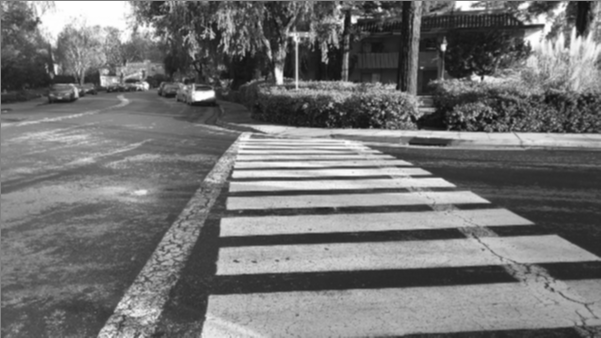
\includegraphics[width=7cm]{SlightlyBlurredInput.png}
\captionfonts
\caption[This is a figure]{Input image blurred and converted to grayscale}
\label{fig:SlightlyBlurred}
\end{center}
\end{figure}

The Sobel derivative is taken in the Y direction, giving us just the changes in the Y direction. These points are either negative or positive, which represents whether they are going from dark to light, or light to dark, giving us pixels that can be either the bottom of the top of the crosswalk. These are potential edges of crosswalks in the image (See figure \ref{fig:TopAndBottomSobel}). 

\begin{figure}[h]
\begin{center}
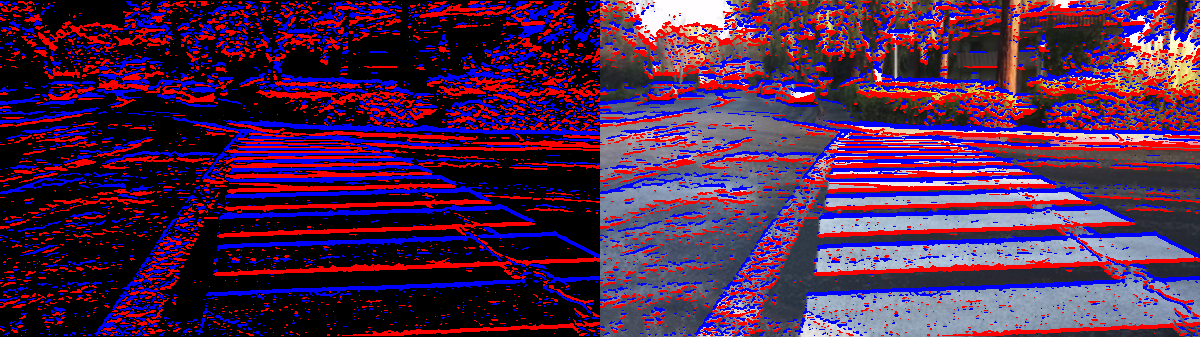
\includegraphics[width=14cm]{TopAndBottomSobel.png}
\captionfonts
\caption[This is a figure]{Sobel derivative of the image - positive values colored red, negative values colored blue}
\label{fig:TopAndBottomSobel}
\end{center}
\end{figure}

Hough line transform is then used to detect lines (figure \ref{fig:HoughLinesAfterMerge}). 

\begin{figure}[h]
\begin{center}
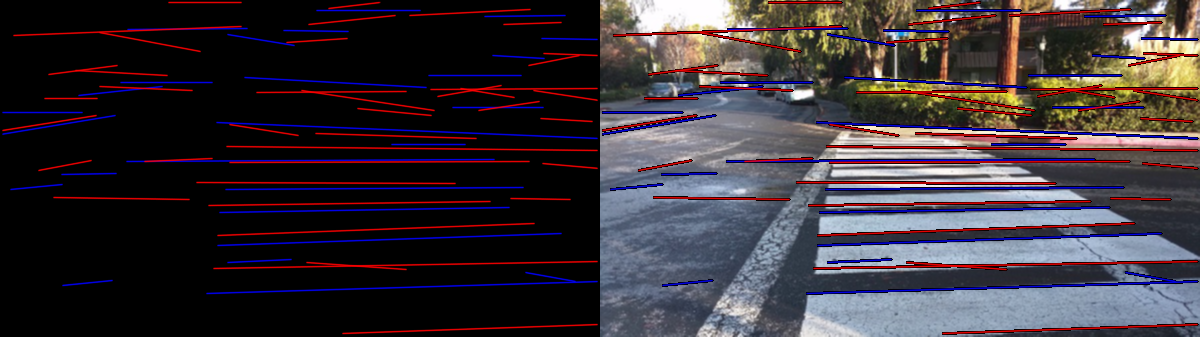
\includegraphics[width=14cm]{HoughLinesAfterMerge.png}
\captionfonts
\caption[This is a figure]{Lines detected using Hough transform on image from figure \ref{fig:TopAndBottomSobel} - blue is potential crosswalk top lines, red is potential crosswalk bottom lines}
\label{fig:HoughLinesAfterMerge}
\end{center}
\end{figure}

The generated lines are either defined as potential crosswalk top edges, or bottom edges. These potential edges are matched up against other edges (top vs bottom edges) to determine if they fit certain criteria to be considered as a stripelet. A stripelet is defined as an area bounded by a top and bottom line that follows certain constraints. The constraints used in Coughlan's figure-ground crosswalk paper \cite{jamesm.coughlanhuiyingshen2006} are the same as used here: Top line is above bottom line in the image, the two lines' slopes are very similar, the vertical width of the generated stripelet is the between a defined cutoff values, and the two lines have sufficient X overlap. If all of these are true, then it is returned as a stripelet (See figure \ref{fig:UnculledStripelets}). 

\begin{figure}[h]
\begin{center}
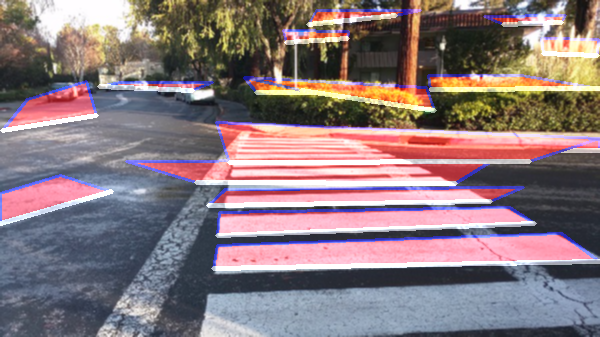
\includegraphics[width=7cm]{UnculledStripelets.png}
\captionfonts
\caption[This is a figure]{All of the stripelets detected after running the constraints on all the input lines from figure \ref{fig:HoughLinesAfterMerge}}
\label{fig:UnculledStripelets}
\end{center}
\end{figure}

\subsection{Neural Network Prediction of Crosswalk Stripelets}

At this point, the algorithm has generated a list of stripelets that are potentially part of the crosswalk. The input for the neural network is a few parameters extracted from the image. The parameters are chosen because they possess characteristics that are believed will contribute to helping identify a stripelet. A couple sample parameters are the stripelet vertical/horizontal width, variance of the pixel intensity, and the lengths of the top and bottom lines. These numbers are calculated and then fed into the trained neural network, resulting in a very fast prediction as to whether or not that stripelet is a crosswalk stripelet.

\subsection{Crosswalk Detection}

The stripelets that are predicted by the neural network to be part of a crosswalk are then checked one by one against the other stripelets through a manual feature comparison process. The compared features of the two stripelets are their average slopes, the horizontal pixel overlap, the vertical width of the stripelets, and the Y range overlap. The average slopes should be similar, the horizontal pixels should have a large amount of overlap, the vertical width of the stripelet lower in the image should be wider, and the Y ranges should have minimal if any overlap. If two of the predicted crosswalk stripelets satisfy all of these these constraints, then the image is declared to have a zebra crosswalk inside of it. If all of the constraints fail to pass, then the image is labeled not a crosswalk. 


\section{Neural}

Once the stripelets are detected, they were all marked as being part of a crosswalk or not. Then assorted types of data about them was computed and saved for the neural network training. Examples of metrics used were lengths of top and bottom of the crosswalk, the difference in length between them, the variance and standard deviation of the pixel intensity, etc. The neural network was then trained with many iterations over the training data. There was a very low chance of a false positive, so 

\section{Identifying crosswalk edges}
Once the neural network was trained, then each stripelet in the image was determined to be likely part of the crosswalk or not. The stripelets determined to likely be part of the crosswalk then had their left and right points run through a RANSAC detection algorithm to pick the best fit line for each side. 
\todo[inline]{CODE NOT YET DONE}
Those lines were then blended across multiple frames in order to attempt a more accurate edge of the crosswalk. 

\chapter{Results}
\label{results}

\todo[inline]{THIS SECTION CURRENTLY NEEDS A NEW CHART, AND THEN EVERYTHING WILL BE ADJUSTED TO ACCOMMODATE THAT}

\todo[inline]{Need a bunch of data here, easy to get}

\todo[inline]{chart for total number of instances and how many were good/bad stripelets}

\todo[inline]{GRAB THE FINAL Numbers}
The training set included 10 input videos and 1000 input frames, which resulted in 8000 stripelets for training. Separate videos were kept to only be used for testing, never for training. There were 10 test videos, totalling in 300 input frames and 2400 detected stripelets. The neural network training of the crosswalk stripelets used many different input parameters to determine the output. The metric used for evaluating these was finding the true positive and false negative rates, as well as the p-value. The true positive rate is calculated by dividing the number of crosswalk stripelets that were predicted correctly as stripelets over the total number of crosswalk stripelets. The false positive rate is calculated by dividing the number of non-crosswalk stripelets predicted as stripelets out of the total number of non-crosswalk stripelets. The P value is found by dividing the number of false positives by the number of stripelets that were predicted to be part of a crosswalk.  The first training parameters tried were:


\begin{enumerate}
   \item Line length of bottom of crosswalk
   \begin{itemize}
     \item This value directly relates to the stripelet measurements.
     \item Crosswalk stripelets would be expected to have certain lengths, so we can hope to gain insight about the validity of the stripelet from this value.
   \end{itemize}
   \item Line length of top of crosswalk
   \begin{itemize}
     \item This value is similar to the bottom length, and this value should pair well with the bottom length to give more information about the stripelet because they are 
   \end{itemize}
\end{enumerate}

\begin{center}
    \begin{longtable}{| l | l | l | l | l |}
    \hline
     & Total & Correct & Incorrect & Prediction Rate \\ \hline
    Part of a crosswalk & \textbf{783} & \textbf{549} & 234 & 549/783 \\ \hline
    Not part of a crosswalk & \textbf{3459} & 3324 & \textbf{135} & 135/3459\\ \hline
    Total Stripelets & 4242 & 3873 & 369 & \\ \hline
    
    \caption{Results from neural network training and prediction using top and bottom length of the crosswalk stripelet}
    \label{tab:Results1-1} 
    \end{longtable}
\end{center}


\begin{longtable}{| l | c |}
  \hline
   & Stripelet Prediction Rate \\ \hline                   
  True Positives & 68.33\%  \\ \hline
  False Positives & 4.39\% \\ \hline
  p-value & .221  \\ \hline

\caption{Results from neural network training and prediction using top and bottom length of the crosswalk stripelet}
\label{tab:Results1-2} 
\end{longtable}


Analysis: These numbers can be very useful, but by themselves will not be very good at determining if a stripelet is part of a crosswalk or not. Two stripelets may have the same values for these measures, but one can be a crosswalk and the other may not be. The results shown in table \ref{tab:Results1-1} and table \ref{{tab:Results1-2} show that we did get a reasonably high rate of true positives, but we still have a 22\% chance that our positive prediction of a stripelet is incorrect. 

Then I decided to try four more parameters:

\begin{enumerate}
   \item Difference in length between the top and the bottom of the stripelet
   \begin{itemize}
     \item This value may assist in giving more value to the difference between the two
     \item We might expect that the difference would help for reasons such as the bottom should always be wider and their difference should usually be a reasonably small number. 
   \end{itemize}
   \item Vertical Stripelet Width
   \begin{itemize}
     \item We would expect that the stripelet vertical width would be a good factor because stripelets should have a certain vertical width that correlates with their top and bottom lengths that would help define them as being part of a crosswalk
   \end{itemize}
      \item Horizontal Stripelet Width
   \begin{itemize}
     \item Same as vertical stripelet width, we would expect the parameters to correlate to others and help them make a match
   \end{itemize}
      \end{itemize}
      \item Vertical Stripelet Location
   \begin{itemize}
     \item The vertical stripelet location (Y value of the stripelet center) should help to correlate with other numbers and give a better prediction. For example, one might expect that a crosswalk stripelet higher in the image would be smaller, so this would correlate with vertical and horizontal stripelet width. 
   \end{itemize}
\end{enumerate}

\begin{center}
    \begin{longtable}{| l | l | l | l | l |}
    \hline
     & Total & Correct & Incorrect & Prediction Rate \\ \hline
    Part of a crosswalk & \textbf{783} & \textbf{419} & 234 & 419/783 \\ \hline
    Not part of a crosswalk & \textbf{3459} & 3324 & \textbf{158} & 158/3459\\ \hline
    Total Stripelets & 4242 & 3743 & 392 & \\ \hline
    
    \caption{Results from neural network training and prediction adding four more values (shown above)}
    \label{tab:Results2-1} 
    \end{longtable}
\end{center}


\begin{longtable}{| l | c |}
  \hline
   & Stripelet Prediction Rate \\ \hline                   
  True Positives & 53.51\%  \\ \hline
  False Positives & 4.57\% \\ \hline
  p-value & .274  \\ \hline
\caption{Results from neural network training and prediction adding four more values (shown above)}
\label{tab:Results2-2} 
\end{longtable}

Analysis: The numbers actually got worse adding these parameters from tables \ref{tab:Results2-1} and \ref{tab:Results2-2}.  ...
\todo[inline]{figure out why}

Then I decided to try four more parameters:

\begin{enumerate}
   \item Variance of the stripelet pixel value
   \begin{itemize}
     \item We would expect this value that represents how much variance is in the pixel values of the images to give the neural network more insight. For example, we might expect crosswalk stripelets to have very minimal variance because the pixels should be mostly uniform
   \end{itemize}
   \item Standard deviation of the stripelet
   \begin{itemize}
     \item This is the square root of the variance, but it may give the same insights that the variance does, and allow a similar but simpler metric for the neural network to use
   \end{itemize}
      \item Standard deviation of the area surrounding the stripelet
   \begin{itemize}
     \item We might expect the area around the stripelet to have a low standard deviation as well because it should be a mostly gray sidewalk
   \end{itemize}
      \item Standard deviation of the area surrounding the stripelet / Standard deviation of the stripelet
   \begin{itemize}
     \item This ratio may help to give the neural network a hint of what their relation could be. 
   \end{itemize}
   \item Average stripelet intensity / average intensity of area surrounding the stripelet
   \begin{itemize}
     \item We would expect that the stripelet intensity would be much greater than the area surrounding it, so this value would assist in finding what ratios are indicative of a crosswalk stripelet or not. 
   \end{itemize}
\end{enumerate}

\begin{center}
    \begin{longtable}{| l | l | l | l | l |}
    \hline
     & Total & Correct & Incorrect & Prediction Rate \\ \hline
    Part of a crosswalk & \textbf{783} & \textbf{637} & 234 & 637/783 \\ \hline
    Not part of a crosswalk & \textbf{3459} & 3324 & \textbf{113} & 113/3459\\ \hline
    Total Stripelets & 4242 & 3743 & 392 & \\ \hline
    
    \caption{Results from neural network training and prediction adding four more values (shown above)}
    \label{tab:Results3-1} 
    \end{longtable}
\end{center}


\begin{longtable}{| l | c |}
  \hline
   & Stripelet Prediction Rate \\ \hline                   
  True Positives & 81.35\%  \\ \hline
  False Positives & 3.27\% \\ \hline
  p-value & .151  \\ \hline
\caption{Results from neural network training and prediction adding four more values (shown above)}
\label{tab:Results3-2} 
\end{longtable}


Final analysis of neural network: Adding all these parameters, we ended up with some rather good results, shown in table \ref{tab:Results3-2} and \ref{tab:Results3-1}. After running the neural network prediction on the output videos, 81.35\% of the crosswalks stripelets were correctly identified as stripelets, with a 3.27\% rate of a positive identification of a crosswalk stripelet being correct. This leaves us with a 15\% chance that a positive ID is incorrect, which is enough to continue with the next step of identifying the image as containing a crosswalk or not. 
\todo[inline]{grab final percentages}

\todo[inline]{Crosswalk identification results}

\todo[inline]{Bounding line results}

\chapter{Future Work}
\label{future work}

\section{Conversion to phone app}

The project was written entirely in the C++ libraries provided by OpenCV, which can be ported easily to a mobile app without many changes. Once the algorithm has access to phone sensors, there are opportunities to implement improvements. The current algorithm assumes that the photos are taken parallel to the horizon, but with access to a phone's sensors, the image frames could be adjusted so that they are guaranteed to be in the correct horizontal orientation. The accelerometer and gyroscope sensors could also be used to help track movement as the user crosses a crosswalk. Using sensors, anything above the horizon line could be discarded \cite{Crosswatch2Lane}. Other mobile technologies such as Project Tango's 3d mapping hardware \cite{projectTango} could be used as well to assist with spatial awareness and other factors such as detecting obstructions that must be avoided. Once the program is converted to a mobile app, there are many interesting ways that it could progress.

\section{Crosswalks with shadows}

As this project did not cover crosswalks with shadows, future work could be done to adapt the algorithm so it can work properly with crosswalks that have shadows inside of them. The current algorithm has difficulties with shadows; one issue is that the Hough line transform might have issues because shadows form strong lines, and another being that some of the neural network training parameters might be drastically different with shadows inside of the stripelets. 

One option might be shadow removal algorithms that would remove the shadows so that the main algorithm doesn't have to account for them at all. This could be a good solution because it would require modifying the current algorithm, but might not the fastest. Shadow removal algorithms are quite common, so there would be many different options \cite{shadowRemoval}. Another potential solution would be to modify the current algorithm to handle the shadows. This method would likely involve modifying the Hough lines grouping, as well as using different or modified training parameters for the neural network, and require additional training data including crosswalks with different types of shadows at various times of day. 

\section{Crosswalks in Extremely Low Light Conditions}

There is a possibility that the neural network method can be adapted to work at night as well. Ideally, this could be accomplished with only extra training data required, but it depends on the camera's low light capabilities. An infrared flashlight or another lighting tool may be required to raise the light level for the crosswalk to be visible. Additionally, a different training set may be required in order to properly work with the crosswalk at night. 

\todo[inline]{not crazy about this section}

\section{More Training Parameters for Neural Network}

The portion of the algorithm that uses neural networks to predict whether or not stripelets are part of the crosswalk would benefit from more investigation into new metrics that would aid the neural network. Investigating new parameters is not a costly procedure in terms of time, and it is not difficult to discover whether a training parameter is working well or not after a single attempt, so it would be worth the investment.  

\section{Edge line detection method improvements}

\todo[inline]{WRITE THIS}

\section{Use Neural network for comparing two stripelets in crosswalk detection}

Currently, the algorithm is using a few different metrics in order to predict whether two stripelets could be a part of the same crosswalk or not. A neural network could be applied to this decision instead, in order to potentially garner a better result. The same parameters that are being manually used currently would be a good starting point for neural network parameters, as well as the other parameters currently being used by the neural network for stripelet prediction. 

\todo[inline]{ADD}

\section{Performance Improvements}

The algorithm contains some areas where the performance could be improved. In this proof of concept, speed isn't as important, so the algorithm is not as optimized as it could be. If it is ported to a phone app, the optimizations would become necessary for a real world usage scenario.
\subsection{Multithreading}
One specific improvement would be to take advantage of multiple CPU cores in order to process multiple frames at the same time. This would improve the throughput and allow greater accuracy due being able to quickly to average the results of frames that are immediately next to each other.
The current implementation running on a decent PC can run at around 1.6 frames per second, and would scale linearly with the number of cores, so if one core is currently 1.6 frames per second, then two cores would be 3.2 frames per second, thus multithreading would give a large performance boost for this application.

\subsection{Finding the Smallest Image Size Necessary}
Another improvement would be to try to find the smallest image size necessary for the algorithm to detect the position of the crosswalk. The smaller the image is, the faster the processing time will be because there are fewer pixels for every operation. This could be discovered by running the algorithm on smaller and smaller crosswalks and finding out when the predictions start degrading to an unacceptable level. The performance would drastically improve, because as the image dimensions are cut in half, the number of pixels are divided by four, which scales almost directly with the runtime because many operations are performed on each pixel, and those operation's runtimes would divided by four. 

\chapter{Conclusion}
\label{conclusion}

\todo[inline]{What I did ( couple sentences), why I did it (more), why I think they worked or didn't work  (biggest)}


% ------------- End main chapters ----------------------

\clearpage
\bibliography{bibliography}
\bibliographystyle{plain}
%\addcontentsline{toc}{chapter}{Bibliography}

\end{document}
